\subsection{LaTeX: Razno}

V tej poglavju so zbrani različni nasveti in triki za delo z LaTeX-om, ki ne sodijo v druge poglavja.

\subsubsection{Obsežnejši projekti}

Za obsežnejše projekte, kot so diplomske naloge, je priporočljivo razdeliti dokument na več datotek in jih vključiti v glavno datoteko z ukazom \texttt{{\textbackslash}input\{\}} ali \texttt{{\textbackslash}include\{\}}.
To omogoča lažje upravljanje in urejanje posameznih delov dokumenta.

Ukaz \texttt{{\textbackslash}include\{\textless pot do datoteke\textgreater \}} vključi vsebino navedene datoteke in samodejno začne novo stran pred in po vključitvi.

Ukaz \texttt{{\textbackslash}includeonly\{\textless ime\_datoteke1\textgreater , \textless ime\_datoteke2\textgreater , ...\}} omogoča vključitev samo določenih datotek med kompilacijo, kar je uporabno za hitrejše pregledovanje določenih delov dokumenta.

\begin{framed}
\textbf{Pazite!}\\
\begin{itemize}
\item Ukaz \texttt{{\textbackslash}include\{\textless ime\_datoteke\textgreater \}} lahko uporabljamo samo v \textbf{telesu glavne datoteke} ne znotraj drugih vklučenih datotek.
\item Ukaz \texttt{{\textbackslash}includeonly\{\textless ime\_datoteke1\textgreater , \textless ime\_datoteke2\textgreater , ...\}} mora biti postavljen v preambulo glavne datoteke.
V telesu dokumenta morajo biti
ukaze \texttt{{\textbackslash}include\{\}} za vse datoteke, ki jih želimo vključiti.
\item Ukaz \texttt{{\textbackslash}include\{\}} vedno začne novo stran, zato ni primeren za vključevanje manjših delov besedila. Poleg tega, ta ukaz ne deluje znotraj okolij, kot so \texttt{{\textbackslash}begin\{figure\}...{\textbackslash}end\{figure\}} ali \texttt{{\textbackslash}begin\{table\}...{\textbackslash}end\{table\}}.
\end{itemize}
\end{framed}

Ukaz \texttt{{\textbackslash}include} je malo omejevalen in ima posebno uporabo: vključiti več poglavje (\texttt{chapter}) v velik projekt. Ta ukaz vedno začne novo stran, to je koristno ko uporabljamo ukaz \texttt{{\textbackslash}indludeonly\{\}}, ker se prelomi strani ne bodo premaknili, če bomo vključili samo določene datoteke.

Včasih je bolj smiselno uporabiti ukaz \texttt{{\textbackslash}input\{\textless pot do datoteke\textgreater \}}, ki vključi vsebino navedene datoteke brez preloma strani.
Ukaz \texttt{{\textbackslash}input\{\}} lahko uporabljamo kjerkoli v dokumentu, tudi znotraj okolij, kot so \texttt{{\textbackslash}begin\{figure\}...{\textbackslash}end\{figure\}} ali \texttt{{\textbackslash}begin\{table\}...{\textbackslash}end\{table\}}.

Ukaz \texttt{{\textbackslash}input\{\}} lahko uporabimo tudi za vključitev datotek z ukazi LaTeX-a, kot so definicije makrov ali nastavitve paketov. Pogosta uporaba je vključitev datoteke, recimo, \texttt{preambula.tex}, ki vsebuje vse nastavitve in pakete, ki jih želimo uporabiti v našem dokumentu.

\begin{framed}
\textbf{Pazite!}\\
Čeprav lahko uporabimo ukaz \texttt{{\textbackslash}input} za naložitev paketov v našo datoteko, mora vrstica, ki vsebuje ukaz \texttt{{\textbackslash}documentclass}, \textbf{vedno} biti v glavni datoteki, pred vsemi ukazi \texttt{{\textbackslash}input}.
\end{framed}

\subsubsection{Barve}

Za uporabo barv v LaTeX dokumentih uporabimo paket \texttt{xcolor}. Paket omogoča uporabo treh ukazov za barvanje besedila ali ozadij:

\begin{itemize}
\item \texttt{{\textbackslash}textcolor[\textless model\textgreater ]\{\textless barva\textgreater \}\{\textless besedilo\textgreater \}}: Barva besedilo z določeno barvo.
\item \texttt{{\textbackslash}color[\textless model\textgreater ]\{\textless barva\textgreater \}}: Spremeni barvo besedila od tega mesta naprej. To je različica \textit{switch} ukaza \texttt{{\textbackslash}textcolor}, kot je ukaz \texttt{{\textbackslash}bfseries} za krepko pisavo (prim. \texttt{{\textbackslash}textbf\{\}}).
\item \texttt{{\textbackslash}mathcolor[\textless model\textgreater ]\{\textless barva\textgreater \}\{\textless matematični\_izraz\textgreater \}}: Barva matematični izraz z določeno barvo. Ne pozabite, da ukaze za \textit{navadno} besedilo običajno ne delujejo v matematičnem načinu.
\end{itemize}

Za zdaj se ne skrbite za neobvezni parameter \texttt{\textless model\textgreater }. Ta parameter nadzira, kaj se pričakuje za argument \texttt{\textless barva\textgreater }. Če ni določen, se privzeto uporablja model \texttt{named}, ki omogoča uporabo vnaprej določenih imen barv, to pomeni, barve pokličemo z imeni.

Barve, ki so vnaprej določene v paketu \texttt{xcolor}, so prikazane v Figure~\ref{tbl:basecolors}.

\begin{figure}[!htbp]
\centering
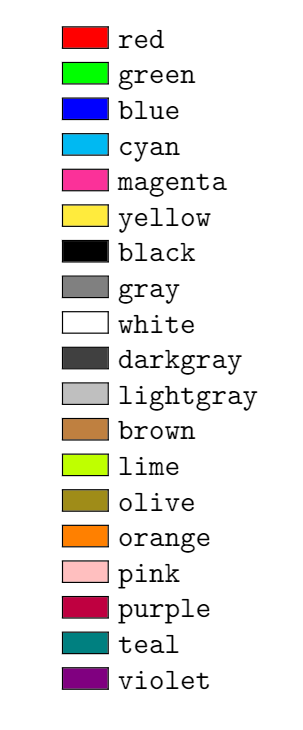
\includegraphics[width=0.7\linewidth]{files/05_xcolorList-efd7422e4e3a9a73a3353c9cd5d66686.png}
\caption[]{Osnovne barve, ki jih določa paket \texttt{xcolor}.}
\label{tbl:basecolors}
\end{figure}

Seznam določenih barv lahko razširimo z uporabo možnosti, ki jih ponuja paket \texttt{xcolor}. Npr z možnostjo \texttt{dvipsnames} lahko uporabimo dodatne barve prikazane v Figure~\ref{tbl:dvipsnames}.

\begin{figure}[!htbp]
\centering
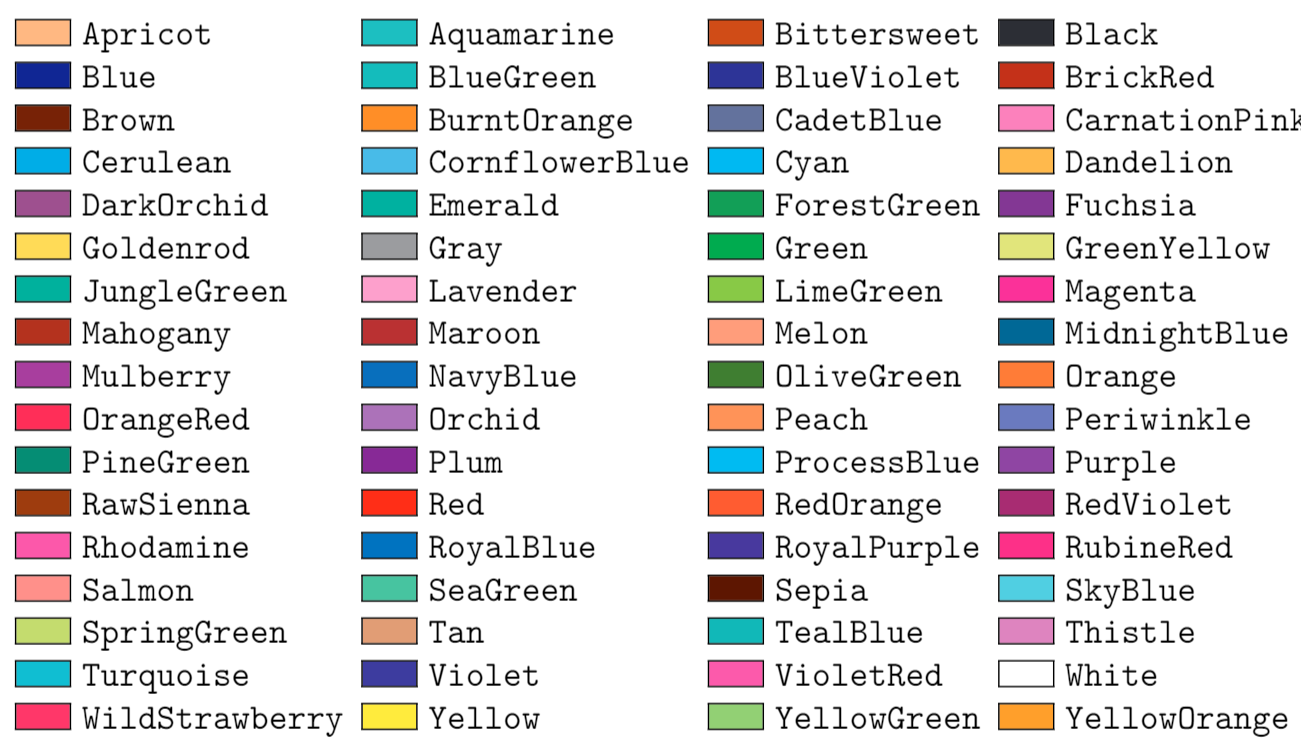
\includegraphics[width=0.7\linewidth]{files/05_xcolorDvipsnames-b995f7f9faffa70345f1476c434c77bc.png}
\caption[]{Dodatne barve, ki jih določa paket \texttt{xcolor} z možnostjo \texttt{dvipsnames}.}
\label{tbl:dvipsnames}
\end{figure}

Druge možnosti so \texttt{svgnames}, \texttt{x11names}. Možnost \texttt{svgnames} določa 151 barv, ki so definirane v SVG standardu, medtem ko možnost \texttt{x11names} določa 317 barv, ki so bile prvotno definirane za X11 Window System. Celoten seznam barv je na voljo v dokumentaciji paketa \href{https://ctan.org/pkg/xcolor?lang=en}{\texttt{xcolor}}.

Drugi način pridobivanja novih barv je z mešanjem dveh ali več barv. Sintaksa za mešanje dveh barv je naslednja:

\begin{verbatim}
<barva1>!<odstotno>!<barva2>
\end{verbatim}

Rezultat je barva, ki je sestavljena iz \texttt{\textless odstotno\textgreater } odstotkov \texttt{\textless barva1\textgreater } in \texttt{(100 - \textless odstotno\textgreater )} odstotkov \texttt{\textless barva2\textgreater }. Na primer, \texttt{red!40!blue} ustvari vijolično barvo, ki je mešanica 40\% rdeče in 60\% modre.

Mešanje lahko vključuje tudi več kot dve barvi. V tem primeru, mešanje je izvedeno zaporedno. Na primer, \texttt{red!50!green!30!blue} najprej zmeša 50\% rdeče in 50\% zelene, nato pa rezultat zmeša z 70\% modre in 30\% prej dobljene barve.

Včasih moramo biti natančnejši pri barvah, ki jih uporabljamo. Za to lahko uporabimo izbirni argument \texttt{model}. Najlažje ga razumemo prek modela \texttt{Gray}. V tem modelu določimo odtenek sive barve z vrednostjo med \texttt{0} in \texttt{15}, kjer \texttt{0} predstavlja črno in \texttt{15} belo.

Podobno lahko uporabimo model \texttt{grey}, kjer vrednosti segajo od \texttt{0} do \texttt{1}, pri čemer \texttt{0} predstavlja črno in \texttt{1} belo.

V Table~\ref{tbl:color-models} so prikazani nekateri barvni modeli, ki jih podpira paket \texttt{xcolor}.

% \begin{table}
% \centering
% \caption[]{Najpogostejši modeli barv v paketu \texttt{xcolor}}
% \label{tbl:color-models}
% \begin{tabular}{p{\dimexpr \linewidth-2\tabcolsep}}
% \toprule
% Model & Osnovne barve/komponente & Razpon parametrov & Primer \\
% \hline
% \texttt{rgb} & Rdeča, zelena, modra & $[0,1]^3$ & \texttt{{\textbackslash}textcolor[rgb]\{1,0,0\}\{Rdeča\}} \\
% \texttt{RGB} & Rdeča, zelena, modra & $\{0, \dots, 255\}^3$ & \texttt{{\textbackslash}textcolor[RGB]\{255,0,0\}\{Rdeča\}} \\
% \texttt{HTML} & Rdeča, zelena, modra & Šestnajstiški zapis & \texttt{{\textbackslash}textcolor[HTML]\{FF0000\}\{Rdeča\}} \\
% \texttt{cmy} & Cijan, magenta, rumena & $[0,1]^3$ & \texttt{{\textbackslash}textcolor[cmy]\{0,1,1\}\{Rdeča\}} \\
% \texttt{cmyk} & Cijan, magenta, rumena, črna & $[0,1]^4$ & \texttt{{\textbackslash}textcolor[cmyk]\{0,1,1,0\}\{Rdeča\}} \\
% \texttt{Gray} & Odtenek sive & $\{0, \dots, 15\}$ & \texttt{{\textbackslash}textcolor[Gray]\{0\}\{Črna\}} \\
% \texttt{gray} & Odtenek sive & $[0,1]$ & \texttt{{\textbackslash}textcolor[gray]\{0\}\{Črna\}} \\
% \texttt{wave} - Valovna dolžina (nm) - $[380,780]$ - \texttt{{\textbackslash}textcolor[wave]\{700\}\{Rdeča\}} \\
% \bottomrule
% \end{tabular}
% \end{table}

\begin{framed}
\textbf{Opozorilo!}\\
Pri mešanju barv v različnih modelih lahko dobimo nepričakovane rezultate. Na primer, da izrazi \texttt{\textless barva1\textgreater !25!\textless barva2\textgreater } in \texttt{\textless barva2\textgreater !75!\textless barva1\textgreater } ne dajeta vedno iste barve, če sta \texttt{\textless barva1\textgreater } in \texttt{\textless barva2\textgreater } definirani v različnih barvnih modelih.
Zato je priporočljivo, da pri mešanju barv vedno uporabljamo barve iz istega modela.
Alternativno v poglavje 6 dokumentacije paketa \href{https://ctan.org/pkg/xcolor?lang=en}{\texttt{xcolor}} najdemo več informacij o spremenjenju med barvnimi modeli.
\end{framed}

Z uporabo ukaza \texttt{{\textbackslash}definecolor\{\textless ime\_barve\textgreater \}\{\textless model\textgreater \}\{\textless parametri\textgreater \}} (v preambuli) lahko definiramo svoje barve. Na primer, z ukazom \texttt{{\textbackslash}definecolor\{ULrdeca\}\{RGB\}\{226,25,30\}} definiramo barvo z imenom \texttt{ULrdeca}, ki je rdeča barva Univerze v Ljubljani.

Doslej smo obravnavali ukaze za barvanje besedila. Možno je tudi spremeniti barbo ozadja strani z ukazom

\begin{verbatim}
\pagecolor[<model>]{<barva>}.
\end{verbatim}

Ta ukaz je različica \textit{switch}, to pomeni da spremeni barvo celotne strani od mesta, kjer je uporabljen, naprej. Če želimo vrniti nazaj privzeto barvo ozadja (prozoren), uporabimo ukaz \texttt{{\textbackslash}nopagecolor}.

V izrazu za barvo lahko uporabimo znak \texttt{-} (minus), da dobimo nasprotno barvo. Na primer, \texttt{-white} predstavlja črno barvo.

Če želimo spremeniti barvo samo določenega območja besedila, lahko uporabimo ukaz \texttt{{\textbackslash}colorbox[\textless model\textgreater ]\{\textless barva\textgreater \}\{\textless besedilo\textgreater \}}.
Ta ukaz obdaja besedilo z ozadjem določene barve.
Ukaz \texttt{{\textbackslash}fcolorbox[\textless model\textgreater ]\{\textless barva\_okvirja\textgreater \}\{\textless barva\_ozadja\textgreater \}\{\textless besedilo\textgreater \}} obdaja besedilo z okvirjem določene barve in ozadjem določene barve.

\subsubsection{Ukazi in okolja po meri.}

LaTeX omogoča ustvarjanje lastnih ukazov in okolij, kar lahko olajša pisanje ponavljajočih se struktur v dokumentu.
Klasični način za definiranje novega ukaza je z uporabo ukaza \texttt{{\textbackslash}newcommand\{\textless ime\_ukaza\textgreater \}[\textless število\_argumentov\textgreater ]\{\textless definicija\textgreater \}} in novega okolja z uporabo ukaza \texttt{{\textbackslash}newenvironment\{\textless ime\_okolja\textgreater \}[\textless število\_argumentov\textgreater ]\{\textless začetek\_definicije\textgreater \}\{\textless konec\_definicije\textgreater \}}.
Čeprav ti ukazi delujejo povsem normalno za osnovne definicije novih ukazov in okolij, bodo postopoma postali zastareli.
Tega pristopa tukaj ne bomo obravnavali, vendar če bralca zanima, priporočamo branje Overleafovih navodil za \href{https://www.overleaf.com/learn/latex/Commands}{nove ukaze}\{target=\_blank\} in \href{https://www.overleaf.com/learn/latex/Environments}{nova okolja}\{target=\_blank\} (v angleščini).

Sodobnejši in bolj zmogljiv način za definiranje novih ukazov in okolij je z uporabo ukaza \texttt{{\textbackslash}NewDocumentCommand} in \texttt{{\textbackslash}NewDocumentEnvironment}.
Ta pristop omogoča bolj fleksibilno določanje argumentov in podpira različne vrste argumentov, kot so obvezni, neobvezni, in več vrst argumentov.

Ukaz \texttt{{\textbackslash}NewDocumentCommand} ima naslednjo sintakso:

\begin{verbatim}
\NewDocumentCommand{<ime_ukaza>}{<vrsta_argumentov>}{<definicija>}
\end{verbatim}

\begin{itemize}
\item \texttt{\textless ime\_ukaza\textgreater }: Ime novega ukaza, ki ga želimo definirati (vključno z \texttt{{\textbackslash}}).
\item \texttt{\textless vrsta\_argumentov\textgreater }: Niz, ki določa vrste argumentov, ki jih ukaz sprejema. To bomo počasi obravnavali v nadaljevanju.
\item \texttt{\textless definicija\textgreater }: Telo ukaza, kjer lahko uporabimo argumente znotraj ukaza.
\end{itemize}

Najlažje ukaz, da lahko definiramo je brez argumentov, to pomeni z praznim nizom za \texttt{\textless vrsta\_argumentov\textgreater }.

Ta način je zelo uporaben, ko obstajajo del besedila ali strukture, ki jih pogosto uporabljamo v dokumentu.
Seveda, če se kdajkoli odločimo spremeniti to besedilo ali strukturo, moramo to storiti samo na enem mestu: v definiciji ukaza.

Pogosta uporaba novih ukazov je pri definiciji matematičnih izrazov, ki jih pogosto uporabljamo. Kot smo videli v prejšnjih poglavjih, nekatere vir (npr. \href{https://www.sist.si/velicine-in-enote-2-del-matematika-sist-en-iso-80000-220196-prevod-v-slovenscino.html}{Standard ISO 80000-2}) priporočajo, da se za matematične konstante in posebne funkcije uporablja rimska pisava (upravičeno).
Seveda, ni smiselno vsakič pisati \texttt{{\textbackslash}mathrm\{{\textbackslash}pi\}} za konstantno $\mathrm{pi}$ ali \texttt{{\textbackslash}mathrm\{e\}} za Eulerjevo število.
Namesto tega lahko definiramo nove ukaze za te konstante:

\begin{framed}
\textbf{Nasvet}\\
Ko definiramo nove ukaze, ki se bodo uporabljali v matematičnem načinu, je priporočljivo, da ne vključimo nobenega simbola, ki označuje matematični način.
Na primer, pri definiciji ukaza za konstantno $\pi$, je bolje definirati ukaz \texttt{{\textbackslash}kpi} kot \texttt{{\textbackslash}mathrm\{{\textbackslash}pi\}} namesto \texttt{\${\textbackslash}mathrm\{{\textbackslash}pi\}\$}.
\end{framed}

Če želimo definirati nov ukaz, ki sprejema argumente, moramo določiti vrsto in število argumentov v nizu \texttt{\textless vrsta\_argumentov\textgreater }.
Nekateri najpogostejši tipi argumentov so prikazani v Table~\ref{tbl:arg-types}.

\begin{table}
\centering
\caption[]{Najpogostejši tipi argumentov v \texttt{{\textbackslash}NewDocumentCommand}}
\label{tbl:arg-types}
\begin{tabular}{p{\dimexpr 0.500\linewidth-2\tabcolsep}p{\dimexpr 0.500\linewidth-2\tabcolsep}}
\toprule
Tip argumenta & Opis \\
\hline
\texttt{m} & Obvezni argument, ki lahko vsebuje več vrstic. \\
\texttt{O\{\textless privzeta\_vrednost\textgreater \}} & Neobvezni argument, ki lahko vsebuje več vrstic. Če ni podan, ima privzeto vrednost \texttt{\textless privzeta\_vrednost\textgreater }. \\
\texttt{o} & Neobvezni argument. Če ni podan, natisne posebni niz \texttt{-NoValue-}. Običajno v definicij uporaba pogojev za preverjanje, ali je bil argument podan kot je ukaz \texttt{{\textbackslash}IfNoValueTF}. \\
\texttt{D\textless levo\textgreater \textless desno\textgreater \{\textless privzeta\_vrednost\textgreater \}} & Neobvezni argument, ki je obdan z \texttt{\textless levo\textgreater } in \texttt{\textless desno\textgreater }. Če ni podan, ima privzeto vrednost \texttt{\textless privzeta\_vrednost\textgreater }. Običajno se uporablja znak \texttt{\textless } in \texttt{\textgreater }, za \texttt{\textless levo\textgreater } in \texttt{\textless desno\textgreater }. Deluje kot \texttt{o}, vendar s posebnimi ločevalniki. \\
\texttt{d\textless levo\textgreater \textless desno\textgreater } & Podobno kot \texttt{D}, vendar brez privzete vrednosti. Deluje kot \texttt{o}, vendar s posebnimi ločevalniki. \\
\texttt{s} & Preklopni argument (switch). Če je prisoten, je vrednost \texttt{{\textbackslash}BooleanTrue}, sicer \texttt{{\textbackslash}BooleanFalse}. Uporabno, ko definiramo ukaze `z zvezdico' ali `brez zvezdice'. \\
\bottomrule
\end{tabular}
\end{table}

Najlažje tip argumenta je \texttt{m}, ki predstavlja obvezni argument. Na primer, lahko definiramo ukaz za barvanje besedila z določenim in barvo. Pri definiciji ukazo, uporabljamo znak \texttt{\#1} za sklicevanje na prvi argument.

Seveda, lahko definiramo ukaze z več argumenti. Dovolj je da dodamo več tipov argumentov v niz \texttt{\textless vrsta\_argumentov\textgreater } in uporabimo \texttt{\#2}, \texttt{\#3}, ... za sklicevanje na druge argumente.

Če želimo definirati ukaz z neobveznimi argumenti, lahko uporabimo tip \texttt{O\{\textless privzeta\_vrednost\textgreater \}}. Ne pozabite, da neobvezni argumenti damo znotraj oklepaj \texttt{[]} pri klicu ukaza.

\begin{verbatim}
Lahko seveda kombiniramo različne tipe argumentov. Na primer, lahko definiramo ukaz z enim obveznim in enim neobveznim argumentom:

::::{grid} 2 2 2 2

:::{card} LaTeX

```latex
V preambuli:
\NewDocumentCommand{\Zap}{O{n}m}
{#2_{1}, \dots, #2_{#1}}
% V telesu dokumenta:
Nekatere zaporedje imajo veliko elementov:
$\Zap[1000]{a}$,
za večino pa sploh ne vemo,
koliko jih je:
$\Zap{b}$.
```

:::

:::{card} PDF

```{figure} ./img/05_eg -ArgsMO -1.png
:label: fig:eg -ArgsMO -1
```

:::
\end{verbatim}

Upoštevajte, da je vrstni red argumentov pomemben. Če je ukaz \texttt{{\textbackslash}ukaz} definiran z vrstnim redom argumentov \texttt{O\{\}m}, ga moramo klicati z obveznim argumentom najprej, nato pa neobveznim argumentom (če ga želimo podati), to pomeni \texttt{{\textbackslash}ukaz[\textless neobvezni\textgreater ]\{\textless obvezni\textgreater \}} je pravilen klic, medtem ko \texttt{{\textbackslash}ukaz\{\textless obvezni\textgreater \}[\textless neobvezni\textgreater ]} ni pravilen klic.
Dobra praksa je, da najprej definiramo vse neobvezne argumente, nato pa obvezne argumente.

Včasih želimo da ukaz deluje drugače, če je neobvezni argument podan ali ne. V tem primeru lahko uporabimo tip argumenta \texttt{o} in ukaz \texttt{{\textbackslash}IfValueTF} za preverjanje, ali je bil argument podan.

Namesto ukaza \texttt{{\textbackslash}IfValueTF}, lahko uporabimo tudi ukaz \texttt{{\textbackslash}IfValueT}, če želimo izvesti dejanje samo, če je bil argument podan, ali ukaz \texttt{{\textbackslash}IfValueF}, če želimo izvesti dejanje samo, če argument ni bil podan. Lahko tudi uporabimo ukaze \texttt{{\textbackslash}IfNoValueTF}, \texttt{{\textbackslash}IfNoValueT}, in \texttt{{\textbackslash}IfNoValueF}, ki delujejo nasprotno.

Ko želimo da ukaz sprejme neobvezni argument z določenimi ločevalniki, lahko uporabimo tip argumenta \texttt{D\textless levo\textgreater \textless desno\textgreater \{\textless privzeta\_vrednost\textgreater \}}.
Običajno se uporabljata znaka \texttt{\textless } in \texttt{\textgreater } kot ločevalnika.

Če namesto \texttt{D\textless levo\textgreater \textless desno\textgreater \{\textless privzeta\_vrednost\textgreater \}} uporabimo \texttt{d\textless levo\textgreater \textless desno\textgreater }, dobimo podoben učinek, vendar brez privzete vrednosti (točno tako, kot ko uporabljamo \texttt{o}). V tem primeru moramo vedno preveriti, ali je bil argument podan z uporabo ukaza \texttt{{\textbackslash}IfValueTF} in podobnih.

Nazadnje, lahko tudi uporabljamo znak \texttt{s} za niz \texttt{\textless vrsta\_argumentov\textgreater }, da definiramo preklopni argument oz. različica ukaz \textit{z zvezdico}. Pri definiciji ukaza, lahko uporabimo ukaz \texttt{{\textbackslash}IfBooleanTF}, da preverimo, ali je bil preklopni argument podan.

Lahko tudi definiramo nova okolja z uporabo ukaza \texttt{{\textbackslash}NewDocumentEnvironment}, ki ima podobno sintakso kot \texttt{{\textbackslash}NewDocumentCommand}.

\begin{verbatim}
\NewDocumentEnvironment{<ime_okolja>}{<vrsta_argumentov>}
{<začetek_definicije>}
{<konec_definicije>}
\end{verbatim}

\begin{itemize}
\item \texttt{\textless ime\_okolja\textgreater }: Ime novega okolja, ki ga želimo definirati.
\item \texttt{\textless vrsta\_argumentov\textgreater }: Niz, ki določa vrste argumentov, ki jih okolje sprejema. To deluje skoraj enako kot pri ukazu \texttt{{\textbackslash}NewDocumentCommand}.
\item \texttt{\textless začetek\_definicije\textgreater }: Koda za začetek okolja, kjer lahko uporabimo argumente znotraj okolja.
\item \texttt{\textless konec\_definicije\textgreater }: Koda za konec okolja.
\end{itemize}

Naslednji primeri naj bi pojasnili uporabo tega ukaza.

\begin{example}\label{eg_okolja_kralj-1}\end{example}Lahko tudi definiramo okolja z argumenti. Na primer, lahko definiramo okolje \texttt{kraljIme}, ki sprejme en obvezni argument za ime kralja.

\begin{example}\label{eg_okolja_kralj-2}\end{example}Tukaj imamo problem, ker želimo imeti različne naslove in zaključke za kralja in kraljico. To lahko rešimo z uporabo preklopnega argumenta \texttt{s}.
Moramo v definiciji okolja uporabiti ukaz \texttt{{\textbackslash}IfBooleanTF}, da preverimo, ali je bil preklopni argument podan; to lahko storimo v obeh delih definicije okolja.

Pazite, za razliko od nekaterih drugih LaTeX okoljih (npr. \texttt{align}), ko uporabljamo okolje z zvezdico, zvezdica gre zunaj oklepajev imenja okolja, t.j. \texttt{{\textbackslash}begin\{kralij\}*\{Ime\}} namesto \texttt{{\textbackslash}begin\{kralij*\}\{Ime\}}. Zvezdica ni potrebna na koncu okolja, t.j. \texttt{{\textbackslash}end\{kralij\}} je pravilen klic tudi za okolje z zvezdico.

\begin{example}\label{eg_kralji}\end{example}\subsubsection{Vaje}\label{05_latexRazno_vaje}

\begin{itemize}
\item Exercise~\ref{ex_input_include}: Vaje o ukazih \texttt{{\textbackslash}input\{\}} in \texttt{{\textbackslash}include\{\}}.
\item Exercise~\ref{ex-gradient}: Vaja o mešanju barv.
\item Exercise~\ref{ex_ukazi}: Vaje o definiciji novih ukazov z \texttt{{\textbackslash}NewDocumentCommand}.
\end{itemize}